% --- Template for thesis / report with tktltiki2 class ---
% 
% last updated 2015/02/03 for tkltiki2 v1.03


\documentclass[english]{tktltiki2}

% tktltiki2 automatically loads babel, so you can simply
% give the language parameter (e.g. finnish, swedish, english, british) as
% a parameter for the class: \documentclass[finnish]{tktltiki2}.
% The information on title and abstract is generated automatically depending on
% the language, see below if you need to change any of these manually.
% 
% Class options:
% - grading                 -- Print labels for grading information on the front page.
% - disablelastpagecounter  -- Disables the automatic generation of page number information
%                              in the abstract. See also \numberofpagesinformation{} command below.
%
% The class also respects the following options of article class:
%   10pt, 11pt, 12pt, final, draft, oneside, twoside,
%   openright, openany, onecolumn, twocolumn, leqno, fleqn
%
% The default font size is 11pt. The paper size used is A4, other sizes are not supported.
%
% rubber: module pdftex

% Line spacing 
%
% Use \linespread{1.3} for "one and a half" line spacing, and
% \linespread{1.6} for "double" line spacing. Normally the lines
% are not spread, so the default line spread factor is 1.
\linespread{1.3}

% --- General packages ---

\usepackage[utf8]{inputenc}
\usepackage[T1]{fontenc}
\usepackage{lmodern}
\usepackage{microtype}
\usepackage{amsfonts,amsmath,amssymb,amsthm,booktabs,color,enumitem,graphicx}
\usepackage[pdftex,hidelinks]{hyperref}
\usepackage[colorinlistoftodos]{todonotes}


% Automatically set the PDF metadata fields
\makeatletter
\AtBeginDocument{\hypersetup{pdftitle = {\@title}, pdfauthor = {\@author}}}
\makeatother

% --- Language-related settings ---
%
% these should be modified according to your language

% babelbib for non-english bibliography using bibtex
%\usepackage[fixlanguage]{babelbib}
\usepackage{natbib}
% \iflanguage{finnish}{\selectbiblanguage{finnish}}{}
 %\iflanguage{english}{\selectbiblanguage{en}}{}
% \selectbiblanguage{english}

% add bibliography to the table of contents
  \usepackage[nottoc]{tocbibind}
  \iflanguage{finnish}{\settocbibname{Lähteet}}{}

% --- Theorem environment definitions ---

\newtheorem{thm}{Theorem}
\newtheorem{lem}[thm]{Lemma}
\newtheorem{cor}[thm]{Corollary}

\theoremstyle{definition}
\newtheorem{definition}[thm]{Definition}

\theoremstyle{remark}
\newtheorem*{remark}{Remark}

% --- tktltiki2 options ---
%
% The following commands define the information used to generate title and
% abstract pages. The following entries should be always specified:

\title{The Planning Problem in Philosophy and Artificial Intelligence}
\author{Pekka Tolvanen}
\date{\today}
\level{Master's Thesis}
\abstract{This thesis concerns philosophy of action and attempts to incorporate a bit of philosophical insight into certain types of software models. Multi-agent systems are used especially in engineering sciences and technology to model the interaction of intelligent agents. They are mostly based on game theoretical frameworks, which are known to be rather limited in their ability to model human interaction. Foundations of social action and cooperation, however, are widely discussed in the philosophy of action and social ontology. How can philosophy then inform multi-agent systems? This thesis explores the question by showing how theories of social action, such as team reasoning, can be applied to multi-agent systems.

I will introduce Michael Bratman's theory of human practical reasoning — the belief-desire-intention framework or BDI for short — and discuss it's applications in software modeling. The BDI framework can be used to model not just single agents, but also multi-agent systems that involve communication and interaction. I will also introduce Raimo Tuomela's account of we-intentions and team reasoning and discuss their possible applications in multi-agent planning as suggested by Raul Hakli. The standard approach to multi-agent modeling begins from the point of view of the individual and builds social action by making the atomistic agents interact together. Planning in the we-mode, however, would enable the agents to begin their planning from the intentions of the group and thus ease the model-building process by reducing the need for communication and improving the ability of human agents and robots to coordinate their actions together.

I will evaluate the benefits and limitations of applying theories of specifically human action to non-human agents. Some of the systems that utilize non-human agents — such as computer programs and robots — aim to represent the action and interaction of real human agents, many interact with people and/or are humanized by people, while others have little or no contact with people. The variety of ways in which multi-agent systems can relate to real people indicates that the usefulness of incorporating elements of human interaction into artificial systems depends on the context of the system in question.}

% The following can be used to specify keywords and classification of the paper:

\keywords{philosophy of science, social ontology, philosophy of action, multi-agent systems}

% classification according to ACM Computing Classification System (http://www.acm.org/about/class/)
% This is probably mostly relevant for computer scientists
% uncomment the following; contents of \classification will be printed under the abstract with a title
% "ACM Computing Classification System (CCS):"
% \classification{}

% If the automatic page number counting is not working as desired in your case,
% uncomment the following to manually set the number of pages displayed in the abstract page:
%
% \numberofpagesinformation{16 pages + 10 appendix pages}
%
% If you are not a computer scientist, you will want to uncomment the following by hand and specify
% your department, faculty and subject by hand:
%
\faculty{Faculty of Social Science}
\department{Department of Political and Economic Studies}
\subject{Social and Moral Philosophy}
%
% If you are not from the University of Helsinki, then you will most likely want to set these also:
%
% \university{University of Helsinki}
% \universitylong{HELSINGIN YLIOPISTO --- HELSINGFORS UNIVERSITET --- UNIVERSITY OF HELSINKI} % displayed on the top of the abstract page
% \city{Helsinki}
%


\begin{document}

% --- Front matter ---

\frontmatter      % roman page numbering for front matter

\maketitle        % title page
\makeabstract     % abstract page

\tableofcontents  % table of contents

% --- Main matter ---

\mainmatter       % clear page, start arabic page numbering

% Write some science here.
\section{Abbreviations}
CDM: Collaborative decision-making
\clearpage

\section{Introduction}


\clearpage
\section{Plans and intentions in philosophy}
The humanity has long been obsessed with the idea of animating the inanimate. Perhaps not surprisingly, guiding action has proven harder than mere animation. Intentional action. Intention guides action. But how to characterize intention? It is crucial to agency.

\subsection{Agency, autonomy and action}
Agents have a capacity to act. The standard conception of agency is intentional action. Philosophy of action strives to say something about the agency. Action is  intentionality

Bratman on temporal agency.
\subsubsection{Free will}
\subsubsection{People are future oriented}
\subsection{Intentions and intentionality}
\subsubsection{Intentions are practical attitudes}
Intentions are practical attitudes as opposed to theoretical and affective attitudes.


Searle: distinction between prospective intention and intention in action (1983, p. 84-85).

Intentions as plans has been Michael Bratman

Intention can be taken to mean at least three things: intention for the future, intention with which and intentional action. A fleshed out account of intention should accommodate for these meanings and their relations.

One of the backbones of Bratman's planning theory is the claim that future-directed intentions are primary to intention-in-action. Bratman argues that first and foremost, intentions are plan states connected to our temporally extended agency. Plans are hierarchically structured so that often plans concerning means are nested in plans concerning ends. These structures are also partial in that they often aren't mapped all the way down; our plans don't have to be detailed all the way to specific acts, even though we might recognize that eventually it will be necessary. \citep*[p.~15]{bratman_shared_2014}

For Bratman, norms of intention rationality descriptively showcase the commonalities of human intentional action and their normative force plays a part in explaining the stability of intentions. \citep*[p.~16]{bratman_shared_2014}

\subsubsection{Philosophy of Mind: what are people like?}
This is an empirical question, answered partly by psychology and cognitive science.
\subsubsection{Philosophy of Action: ??}
\subsubsection{Ethics: which acts are intentional?}
\subsubsection{Do intentions constrain choice? (Bratman vs Sinhababu)}
Michael Bratman’s theory of human practical reasoning \citep{bratman_intention_1987, bratman_shared_2014}, Belief-Desire-Intention or BDI for short, has already greatly influenced model building in computer science in the field of artificial intelligence, in which it is often implemented as the belief–desire–intention software model. Bratman's model is an extension of the Belief-Desire, or BD model, which is widely used especially in game theory. Intentions are desires that the agent has already chosen to do, based on his beliefs.

\subsubsection{Is intention needed at all?}
Sinhababu argues that the belief-desire model can account for intention, thus Bratman's intention isn't needed at all.

But how does a desire give birth to a belief that we will eventually do what we want? Sinhababu doesn’t explicate the mechanism. Granted, any psychological mechanism could be easily added into the account. There could be some circularity though: “All that matters for exclusion is that when we intend to do something in the future, we form the belief that we’ll do it.”
As a causal claim this would be circular: an intention (an intentional desire perhaps) leads to a corresponding belief and at the same time a desire qualifies as an intention only with the corresponding belief. As a requirement.
Exclusion doesn’t have to be a fact, it can be a norm. This allows for failure.

Even if Sinhababu is right, there seems to be something alluring about the concept of intention. Do beliefs about our own plans differ from other kinds of beliefs? Their truth-values depend on facts, but crucially their truth also hangs on our own resolve. It’s very much in our own hands. In some sense they are very fidgety: in one second they can be true, and false in another.
Is a bad plan still a plan?

Bratman:
As Bratman (1999, p. 15) notes, the desire-belief model articulates a normative conception of practical rationality at the same time as it attempts to describe the piece of the human mind relevant to intuition and action.

Volitional commitment
Conduct-controlling pro-attitudes vs potential influencers of action
“settling”
According to Sinhababu if desire-belief pairs are sufficient for motivation they are conduct-controlling. However, Bratman does make a distinction between conduct-controlling pro-attitudes and pro-attitudes as potential influencers of action. Motivation for Sinhababu seems to be a potential influencer rather than conduct-controlling (Sinhababu 2013, footnote 25). This alone makes the point somewhat moot.
Furthermore, related to the previous issue, Bratman’s point (which Sinhababu fails to see “If there’s some problem with desire-belief pairs controlling conduct, Bratman hasn’t told us what it is” even when he quotes Bratman on settling) is that having a desire and a relevant means-ends belief doesn’t settle the issue. According to Sinhababu’s account, we act on our strongest motivation, the highest combined (calculated) means-ends probability and the strength of our desire. Bratman acknowledges that having a desire and a corresponding belief provides a reason to act, but also claims that it doesn’t settle the issue. Acting on our strongest motivation would surely be rational, but people are not always rational (though I think Sinhababu says so in his paper as well). Sinhababu’s account thus seems more normative than descriptive.
“In requiring that I desire to go more than I desire to perform actions thought incompatible with going, the account makes it impossible to intend to perform actions thought incompatible. But while it is, other things equal, criticizably irrational to have such conflicting intentions, it does seem possible to be guilty of such irrationality. And we want our theory to allow for this possibility.” Bratman p. 19
Two kinds of beliefs: 1) means-ends belief about the possibility of the intended issue and 2) a belief about my future actions.

\subsection{Collective intentionality}
BRATMAN

Bratman's central contribution is his theory of collective intentionality. Another difference between theories is the location of collectivity in collective intentions, where in the intention does the collectivity reside. Content, mode and subject.

For Bratman collectivity is in the content of intentions: "I intend that we J." For Bratman collectivity also requires common knowledge and more than one people intending that we J with meshing subplans. The benefits of situating collectivity into the content of intentions are...

Intended plans, into which the agent is committed, are 1) driving factors of means-end reasoning, 2) constraints on options, and also 3) influence beliefs about the future \citep*[p.~9]{bratman_plans_1988}. Or are committed plans real beliefs rather than just things that influence beliefs? \todo[inline]{on second thought, nah, why would they be beliefs?}

Of course at least in the planning process and probably later too, plans are weaker than beliefs. While a change of belief can make a plan impossible, a plan can't change in a way that would make beliefs impossible. This might be just due to the fact that plans are always about the future. Another, maybe bigger, factor is of course the fact that I am relatively free to change my plans (Or am I really? Maybe this is just due to the fact that they are in the future. Of course some empirical facts can be changed by the agent as well, thus changing the belief as well.), but if I want to be rational, I can't change my beliefs.
\todo[inline]{An intriguing subject: the difference between beliefs about past, present and future.}

To constrain, plans must be stable. To be stable, plans (especially about the far future) need to be partial (temporally and/or structurally). Structural partiality of plans allows for their decomposition into intentions. Eventually agents "fill in" their partial plans.

This analysis is super interesting since it seems to show the very real differences between people. I think that a big factor of conflict in relationships is that some people allow for way more partiality in their plans than others. One resulting problem is that to the stringent partner the requirement of consistency is often violated, whereas to the non-stringent partner the available options are unnecessarily constrained. Neither has to be overly stringent or overly non-stringent. \citep*[p.~20]{bratman_plans_1988} use similar terms, \textit{cautious} and \textit{bold}, to denote the treshold of the filter override (I guess this is not the same thing I discussed above?). 

The requirement of consistency (or means-ends coherence) in plans as a way of means-ends reasoning seems to lead inevitably to the role of plans as a constraint.

SEARLE AND TUOMELA

For Searle and Tuomela, collectivity resides in the mode of the intention. The mode of we-intentions is collective whereas the mode of I-intentions is not. We-intentions are intentions about us. A group has a joint intention if the agents in the group have similar we-intentions and mutual belief. The benefits of situating collectivity into the mode of intentions are...

GILBERT

For Margaret Gilbert, collectivity resides in the subject of intentions (or commitments): if A and B have a joint commitment, they constitute a plural subject that is the subject of the commitment.

\section{Planning in AI}

AI is the study of rational action, which means that planning is important, "devising a plan of action to achieve one's goals".

According to this definition planning seems like straightforward means-ends reasoning. Bratman however differentiates means-ends reasoning from intention. Two conceptions of a plan. The Plan Library is a subset of the agent's beliefs \citep[p.~7]{bratman_plans_1988}, a set of (contrafactual?) conditionals. A plan is an adopted plan.

Thus it seems that planning can be the formulation of means-ends beliefs or conditional contrafactuals, in other words compiling a plan library. Or it can be the process of adopting/discarding plans as intentions. These take place in different places of the architecture diagram \citep[p.~7]{bratman_plans_1988}.

An architecture for resource-bound agents \citep[p.~7]{bratman_plans_1988} has input in perception that changes beliefs.

\subsection{The interdisciplinary field of AI}
Computer science, cognitive science...
\subsection{The planning problem}
In the field of AI, or artificial intelligence, the planning problem or the problem of automating means-end reasoning, is central when it comes to rational behavior. It is a formalized, algorithmic, mathematical excercise. In multi-agent systems formulating the preconditions, the assumptions, have common ground with many philosophical questions. In what sense might groups have plans and how do groups plan? How do individuals take groups and their (social) environment in general into account in or in the making of their plans? Multi-agent planning raises many questions about how individualist the world is and how individualist we should be.

Another problem: planning at higher levels of abstraction.

Planning can occur before or during the execution of the plan.

\subsection{Autonomous agents and complexity}

\subsubsection{Artificial agents}

Future oriented? Autonomous agents as opposed to functional systems that merely compute.

According to Wooldridge \citeyearpar[p.~8]{wooldridge_intelligent_2013} (following \citealt{wooldridge_intelligent_1995}), an agent is defined as "a system that is situated in some environment and that is capable of autonomous action in this environment in order to achieve its delegated objectives". Autonomy "is used to mean that agents are able to act without the intervention of humans or other systems: they have control both over their own internal state and over their behavior." Environments can be deterministic or non-deterministic, accessible or inaccessible, episodic or non-episodic, static or dynamic and finally discrete or continuous \citep[p.~6]{wooldridge_intelligent_2013}. Capability to act in an environment presupposes sensors for input in the form of percepts about the environment, and effectors or actuators to interact with the environment. To be able to act in all but the most trivial environments, they must be robust enough to withstand failure.

An intelligent agent is defined by Wooldridge \citeyearpar[p.~8]{wooldridge_intelligent_2013} as an agent that behaves proactively, reactively and socially in order to meet its delegated objectives. I presume that an ability to behave in such a manner is enough to satisfy the requirements of an intelligent agent. The intelligent agent can act in environments that are more complex, with uncertainty or with multiple agents capable of changing the environment.

* What does it mean that it's easy to build purely reactive systems? \citep[p.~9]{wooldridge_intelligent_2013} 

* What about the ability to dissect a goal to small, executable pieces? I guess that's really what we mean by proactiveness.

The hard part in building intelligent agents is the balance between a goal-directed system and a purely reactive system. This means that we don't want the agent to continually respond to the environment forgetting its goals. To be exact, this is already in the definition of reactivity: "in order to satisfy their delegated objectives" \citep[p.~8]{wooldridge_intelligent_2013} . Perhaps it should be omitted in order to produce the conflict between goal-directedness and reactiveness.

A big part of excessive reactiveness in humans is also being reactive to one's own internal states that one does not have direct control of, such as emotions, etc.

Finally, cooperation means not just any interaction, but the ability to negotiate and cooperate.

\textbf{Autonomy}: more usually than not, we don’t want managing a system to be a game of Lemmings, where the agents are predictable, but doomed to fail if not swiftly assisted through the various obstacles in their environment.

One factor related to autonomy is the ability to function in different environments. It’s robustness, it’s ability to withstand (and function in) a variety of environments, that are might not be specified in the beginning. This is close to reactivity \citep[p.~8]{wooldridge_intelligent_2013} .

\textbf{Transparency}: not having to reverse-engineer the system on the run in order to use it efficiently, or aid it. This is often related to human capacities and human-likeness.

\subsection{Constraining choice}
The problems of unbounded single-agent models

The need for simplificatory assumptions is often present in any model-building exercise. The main factor on most cases is our resource-boundedness. In most cases even if time is not crucial for any other reason, the environment might change in a way that demands more practical reasoning, more processing and thus more time. It allows for complexity in the form of multiple agents, changing environment.

Practical reasoning under constraint might not be desirable, but it is realistic in that every system on the planet does that. This might lead one to think that a good way is to emulate the ways living systems have adapted to reason practically under constraint. This is problematic at least for the following reasons: 1) in most / the most interesting cases we don't know exactly how living systems work, 2) there might be better ways to cope with resource-boundedness and 3) the environment for many if not most artificial agents is not similar to us and 4) the way of perceiving the world of artificial agents can differ and thus lead to different ways of parsing and arranging the concepts relevant to action.

In the architecture suggested by Bratman, Israel and Pollack \citeyearpar{bratman_plans_1988} plans constrain the amount of practical reasoning the agent must do.

In my opinion, the motivation or the goal of Bratman, Israel and Pollack in their 1988 paper was to refine such simplificatory assumptions that might trump in some aspects the much researched single-agent models.

\subsubsection{Practical reasons, tractability}
Tractability is also discussed in the  philosophy of economics.

Raimo Tuomela's theory of social action is based on the notion of we-mode. He considers acting in the we-mode as action that is motivated by the supposed intentions of any social group we belong to. Acting in I-mode, on the other hand, begins from our own intentions. Raul Hakli (forthcoming) suggests that Tuomela's we-mode thinking could be used in designing multi-agent models of artificial intelligence. According to Hakli, the standard approach is to begin from the point of view of the individual and try to build social action by making the atomistic individuals interact together. Planning in the we-mode however would enable the individuals to begin from the intentions of the group and thus ease the model-building process.

\subsubsection{Intentions}

The BDI-framework based on Bratman's work in the philosophy of social action has been adopted to AI.

Here I present some notable differences between the work of Michael Bratman and other theorists and try to evaluate if these differences are relevant to the theories' application in AI, hoping to find stuff that has been overlooked. Bratman's work is individualist and reductive which might to an extent help in the creation of implementable formalizations.

\subsection{Modeling, alogrithms}




\clearpage
\section{Contingency of intentions in humans and usefulness of intentions in AI}


\subsection{Possibility of different intentionalities in non-humans}


\subsubsection{Non-constraining intentionalities (Sinhababu)?}


\subsubsection{Ethically irrelevant intentionalities (Free will, Mele)}


\subsection{Also useful because makes machines more relatable and predictable for humans}

"Reduced need for communication, bargaining and argumentation" "may lead to more human-like behaviour and therefore make it easier for humans to interact with robots – improved ability to coordinate their actions with human beings" "behaviour that -- appears familiar to human partners" (Hakli forthcoming)

\subsubsection{Team reasoning and other planning methods}
"Also partial global planning (PGP) methods..." (Hakli forthcoming)

The difference between team reasoning and "a bottom-up strategy of starting from the plans of individual agents and then [using] some sort of plan merging method to coordinate them into a global plan" (Hakli forthcoming (or similar) springs to mind the possible way agents and groups go about forming their group intentions: by recognizing group intentions and group goals, comparing them to one's own and joining groups with similar goals or goals that resonate in some other manner with one's own values, feelings, beliefs, desires, intentions.


\subsection{Intentionality helps make machines moral?}


\section{The planning problem}
In AI and in philosophy. A philosophical take on the planning problem. What is problematic in planning or what problem(s) does planning solve? Several problems, why did I choose the definition I chose?

"Who plans the planner?" It's well known that even decision making by majority can lead to opposite results depending on the decision-making process (Pettit?).


\section{Empirical/philosophical vs practical interest toward intentions (and everything)}
There is some common ground between theory of social action and multi-agent systems. There are also differing goals, etc. Both fields are interdisciplinary, drawing from a variety of disciplines. This work is also interdisciplinary, an attempt of interdisciplinary integration.

What does it mean to have pragmatist goals / interests? Might want to check Stanford Encyclopedia.

Differing goals in the philosophy of social action and AI-related research. It goes almost without saying that the goals of AI research are more practical or pragmatic while the goals of philosophy are usually characterized as epistemic. What does this mean? On a finer mesh, one can strive towards e.g. formalization or implementation. These are not exclusive, on the contrary they can support each other: formalization can and usually will aid in implementation. Pragmaticity and epistemicity are not exclusive either, but they clearly seem to be different goals. Either the goal is pragmatic, epistemic or both, but striving toward a purely epistemic goal will not advance pragmatic goals except by accident.

So formality, implementation are goals, where pragmaticity, epistemicity are kinds of goals?

Why do the scientists see these as promising? The reasons might have to do with computation or modelling, formalization which might have further applications in automatization, pragmatic reasons. I would describe some of the aforementioned as pragmatic reasons. The same goals can be epistemic as well. The goals of the social theorists are probably epistemic.

Constraining "the amount of further practical reasoning she must perform." \citep*{bratman_plans_1988}.


\section{Multi-agent systems and collective intentionality}
Misselhorn (2015) suggests applications of philosophical cooperation and collective agency for multi-agent systems in engineering, robotics, computer science and AI.

\subsection{Individualist vs collective frameworks in AI}

A theoretical argument for using collective rather than individualist frameworks in AI could be that we use abstract conceptual thinking as a way to lessen our cognitive workload. Levels of abstraction. The use of collective concepts is thus very important to us.




\subsection{Notes from Panzarasa}
Notes from \citeauthor{panzarasa_formalizing_2002}
A formal architecture built on top of \citet{wooldridge_intelligent_1995} with more nuanced social stuff.

p. 105 “High-level formal architecture for decision-making within a social context” with a hint of an implementation architecture.

p. 58 “Both individualistic and higher-order units of analysis and constructs are needed” (viitteet 5, 16, 17, 55, 63)): “individual agents both create and are products of social interaction”

p. 59 “to capture the dynamics of making a decision within a social setting we need representations that address higher-order units of analysis (i.e. groups, multi-agent actions, joint doxastic, motivational and deontic attitudes).

p. 79 The model is idealized (e.g. sequentiality).

p. 56 “we need to re-consider and extend our notions of practical reasoning and decision-making so that they deal with the inherently social aspects of these classes of multi-agent systems” ja p. 56 “CDM has generally been viewed and modelled as a kind of distributed reasoning and search, whereby a collection of agents collaboratively go through the search space of a problem in order to find a solution.” <- onko tämä siis “inherently social”? Ei jotenkin kauheen sosiaalinen kuvaus.

pp. 86 and 89 imply that intention is not commitment vs. \citealt{cohen_intention_1990} ”Intention is Choice with Commitment”


\subsection{Joint commitments and democracy theory}

\section{Constraining vs guiding choice (Bacharach) compered to top-down vs bottom-up solving in planning}

\clearpage
\section{Interdisciplinary aspects}
\clearpage


%\begin{figure}
%\centering
%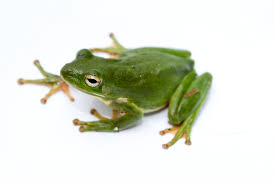
\includegraphics[width=\textwidth]{frog}
%\caption{Caption for the image.}
%\end{figure}

% --- References ---
%
% bibtex is used to generate the bibliography. The babplain style
% will generate numeric references (e.g. [1]) appropriate for theoretical
% computer science. If you need alphanumeric references (e.g [Tur90]), use
%
% \bibliographystyle{babalpha-lf}
%
% instead.

\clearpage

%\bibliographystyle{babplain-lf}

\bibliographystyle{apalike}
\bibpunct{(}{)}{;}{a}{,}{,}
 \bibliography{Zotero.bib}



% --- Appendices ---

% uncomment the following

% \newpage
% \appendix
% 
% \section{Example appendix}

\end{document}